% !TEX TS-program = pdflatex
% !TEX encoding = UTF-8 Unicode

\documentclass[11pt]{article}
\usepackage[utf8]{inputenc} 
\usepackage[parfill]{parskip}
\usepackage[T1]{fontenc} 

\usepackage{fixltx2e}
\usepackage{calc}
\usepackage{doxygen}
\usepackage[export]{adjustbox} % also loads graphicx
\usepackage{makeidx}
\usepackage{multicol}
\usepackage{multirow}
\PassOptionsToPackage{warn}{textcomp}
\usepackage{textcomp}
\usepackage[nointegrals]{wasysym}
\usepackage[table]{xcolor}

\usepackage{csvsimple}

% Font selection
\usepackage[T1]{fontenc}
\usepackage[scaled=.90]{helvet}
\usepackage{courier}
\usepackage{amssymb}
\usepackage{sectsty}
\renewcommand{\familydefault}{\sfdefault}
\allsectionsfont{%
	\fontseries{bc}\selectfont%
	\color{darkgray}%
}
\renewcommand{\DoxyLabelFont}{%
	\fontseries{bc}\selectfont%
	\color{darkgray}%
}
\newcommand{\+}{\discretionary{\mbox{\scriptsize$\hookleftarrow$}}{}{}}

%%% PAGE DIMENSIONS
\usepackage{geometry} % to change the page dimensions
\geometry{a4paper} % or letterpaper (US) or a5paper or....
\geometry{margin=1in} % for example, change the margins to 2 inches all round

\usepackage{graphicx} % support the \includegraphics command and options
\usepackage[parfill]{parskip} % Activate to begin paragraphs with an empty line rather than an indent

%%% PACKAGES
\usepackage{booktabs} % for much better looking tables
\usepackage{array} % for better arrays (eg matrices) in maths
\usepackage{paralist} % very flexible & customisable lists (eg. enumerate/itemize, etc.)
\usepackage{verbatim} % adds environment for commenting out blocks of text & for better verbatim
\usepackage{subfig} % make it possible to include more than one captioned figure/table in a single float
% These packages are all incorporated in the memoir class to one degree or another...
\usepackage{graphicx} 
\graphicspath{ {./images/} }

\usepackage{ifpdf}
\ifpdf
\usepackage[pdftex,pagebackref=true]{hyperref}
\else
\usepackage[ps2pdf,pagebackref=true]{hyperref}
\fi
\hypersetup{%
	colorlinks=true,%
	linkcolor=blue,%
	citecolor=blue,%
	unicode%
}


%%% HEADERS & FOOTERS
\usepackage{fancyhdr} % This should be set AFTER setting up the page geometry
\pagestyle{fancy} % options: empty , plain , fancy
\renewcommand{\headrulewidth}{0pt} % customise the layout...
\lhead{}\chead{}\rhead{}
\lfoot{}\cfoot{\thepage}\rfoot{}
%%% END Article customizations

%%% The "real" document content comes below...

\title{Analiza Algorytmów - Projekt}
\author{Stawczyk Przemysław 293153}
\date{} % Activate to display a given date or no date (if empty),
         % otherwise the current date is printed 


\begin{document}
	  \hypersetup{pageanchor=false,
		bookmarksnumbered=true,
		pdfencoding=unicode
	}
	\maketitle
	\setcounter{secnumdepth}{3}
	\setcounter{tocdepth}{3}
	\tableofcontents
	\clearpage

\section{Opis Zagadnienia}
\subsection{Zadane polecenie}
    Detektyw Karczoch poszukuje nieuczciwych kont na instagramie. Do tego celu analizuje komentarze dotyczące zamieszczanych zdjęć — wie, że takie konta często walczą między sobą, kupując zwolenników i malkontentów. W komentarzach do takich kont, ludzie z jednej grupy piszą tylko do ludzi z drugiej i odwrotnie. Detektyw Karczoch wie, że zwolennik nigdy nie rozmawia z innym zwolennikiem, a malkontent z malkontentem - to dla nich strata czasu.\\
    
	Zadanie : \textsl{Przygotować program, który na podstawie zamieszczonych komentarzy oceni, czy dane konto jest nieuczciwe.}

\subsection{Przykładowe dane wejściowe}

\paragraph{Uczciwe :}
\begin{texttt}\\
  \#Jan: Piękne zdjęcie.\\
  \#Ola: @Jan Masz rację.\\
  \#Ania: @Ola Nie ma racji!\\
  \#Jan: @Ania właśnie, że mam!\\
  \#Ola: @Ania sama nie masz!\\
\end{texttt}
\paragraph{Nieuczciwe : }
\begin{texttt}\\
   \#Jan: Piękne zdjęcie.\\
   \#Ola: @Jan Nieprawda.\\
   \#Jan: @Ola czemu tak twierdzisz?\\
   \#Ania: @Ola no właśnie?\\
   \#Tomek: @Ania twierdzi tak, bo ma rację!!!\\
\end{texttt}
\subsection{Założenia}
\begin{itemize}
\item
Zakładam, że treść komentarza nie ma znaczenia więc dla opisanego celu liczy się jedynie adresat komentarza.
\item
Zakładam, że pojedynczy komentarz może nie mieć adresata lub mieć dokładnie jednego adresata.
\item
Zakładam, że istnienie pojedynczych komentarzy od osób które nie adresują do nikogo komentarzy ani nie są adresatami żadnego komentarza nie ma znaczenia dla rozstrzygnięcia uczciwości konta
\end{itemize}

\section{Koncepcja Algorytmu}
\subsection{Używane pojęcia}
Przy opisie algorytmu stosuje następujące odwzorowanie:
\begin{itemize}
\item
Każdy komentujący jest reprezentowany przez wierzchołek grafu.
\item
Komentarz adresowany do innego użytkownika jest reprezentowany przez krawędź w grafie.
\item
Wiele komentarzy pomiędzy dwoma użytkownikami \textbf{nie} jest odwzorowane jako wielokrotne krawędzie lub krawędzie ważone.\\
 \textsl{Istotny jest fakt komunikacji 2 komentujących, a nie jej objętość}
\item
Komentarz jest odwzorowany jako krawędź nieskierowana. \\
\textsl{Istotny jest fakt komunikacji 2 komentujących, a nie który z użytkowników napisał do którego}
\end{itemize}
\subsection{Zarys działania}
\paragraph{Opis :\\}
   Proponowany algorytm opiera się na założeniu, że istnienie 2 grup \textsl{[zwolenników i malkontentów]}, które nie piszą komentarzy wewnątrz swoich grup jest równoznaczne z możliwością podzielenia wierzchołków grafu na 2 części w których nie ma krawędzi \textsl{[dwudzielność grafu]}.\\ Pojedyncze wierzchołki\textsl{[użytkownicy którzy nie piszą do nikogo, ani nie są adresatami wiadomości]} nie mają znaczenia dla rozstrzygnięcia dwudzielności grafu.
\paragraph{Szkic kroków}
\renewcommand{\labelenumi}{\arabic{enumi}}
\begin{enumerate}
\item
Wczytanie listy komentarzy ze standardowego wejścia \textit{[do napotkania znaku nowej linii, można wysłać za pomocą crtl+D]} lub pliku.
\item
Z problemu tworzony jest graf identyfikowany nazwami użytkowników
\item
Usunięcie pętli [połączeń z wierzchołka do niego samego], wierzchołków nieposiadających oraz powtarzających się krawędzi [np poprzez niedodawanie ich do grafu wynikowego]
\item
Przejście po wierzchołkach "kolorując" je na przeciwne kolory zaczynając od dowolnego niepokolorowanego. Następne wierzchołki brane z kolejki.
\renewcommand{\labelenumii}{\Roman{enumii}}
\begin{enumerate}
\item
Koloruj wierzchołki sąsiednie na przeciwny kolor. Umieść niepokolorowane wcześniej wierzchołki w kolejce do odwiedzenia.
\item
Gdy wierzchołek po drugiej stronie krawędzi jest w tym samym kolorze: \\
\textit{Znaleziono nieparzysty cykl w grafie co jest równoznaczne z faktem, że graf nie jest dwudzielny}\\
STOP --> \textsl{Konto jest uczciwe.}
\end{enumerate}
\item
Usuń pokolorowane wierzchołki.
\item
Jeśli graf niepusty: idź do 3 --> \textsl{Przetwarzanie kolejnego spójnego podgrafu},\\ jeśli pusty: \\
\textit{Udało się pokolorować graf kolorowaniem dwubarwnym wiec jest on dwudzielny.}\\
KONIEC --> \textsl{Konto nie jest uczciwe}
\end{enumerate}
\subsection{Złożoność Algorytmu}
\subsubsection{Analiza Złożoności Algorytmu}
Algorytm iteruje po wszystkich wierzchołkach, a w ramach każdego z wierzchołków po wszystkich jego krawędziach.\\
Z tego wynika, że złożoność pesymistyczna algorytmu powinna być klasy \textit{O(V+E)}, gdzie \textit{V} to ilość wierzchołków, a \textit{E} ilość krawędzi w grafie.
\subsubsection{Przyjęta koncepcja pomiarów}
Algorytm w przypadku konta uczciwego może zakończyć się wcześniej, więc aby sprawdzać złożoność algorytmu należy mierzyć czasy wykonania analizy nieuczciwych kont. Aby profilować sam algorytm, mierzony powinien być jedynie czas spędzony na obliczeniach więc będzie on mierzony dopiero po wczytaniu całego grafu z pliku do pamięci. \\\\
Dla wybranych wielkości grafu mierzony byłby czas dla kilku danych testowych. Analiza byłaby wykonana osobno ze względu na ilość krawędzi \textsl{[przy stałej ilości wierzchołków]}, oraz na ilość wierzchołków \textsl{[przy stałej ilości krawędzi, jednak większej od liczby wierzchołków]}.
\section{Założenia Implementacyjne}
\subsection{Technologie planowane do wykorzystania}
\begin{itemize}
\item
\textsl{C++} jako język do implementacji struktury grafu i algorytmu.
\item
\textsl{Mersenne Twister} jako generator liczb losowych na potrzeby generacji danych, implementacja z biblioteki standardowej
\item
Program do generowania plików z komentarzami zintegrowany z głównym programem
\item
\textsl{boost::chrono} w celu pomiaru czasu spędzonego przez algorytm na procesorze. 
\item
\textsl{CMake} jako narzędzie do zarządzania projektem i jego budowaniem
\end{itemize}
\subsection{Struktury danych}
\begin{itemize}
\item
"Node" - \textsl{jako klasa zawierająca nazwę użytkownika, pole określające kolor, identyfikowana przez numer pozycji w dynamicznej tablicy}
\begin{itemize}[\textsl{W Node} :]
\item
vector<int> - \textsl{przechowuje wierzchołki sąsiednie.}
\item
enum "Kolor" - \textsl{określa czy wierzchołek był odwiedzony oraz kolor odwiedzonego wierzchołka.}
\end{itemize}
\item
map<String, int> - \textsl{zapewniająca odwzorowanie nazwy użytkownika na pozycję w tablicy} \\ 
\textsl{Pomocniczo przy wczytywaniu grafu}
\item
vector<Node> - \textsl{kontener przechowujący wierzchołki}\\ 
\textsl{Zapewnia dostęp do wierzchołka poprzez numer} 
\item 
list<int> - \textsl{przechowuje listę wierzchołków do odwiedzenia, umieszczane są w niej kolejni nieodwiedzeni sąsiedzi przetwarzanego wierzchołka}
\end{itemize}
\section{Generowanie danych wejściowych}
\subsection{Parametry}
\begin{itemize}
\item
liczebność wierzchołków w grafie lub liczebność obu grup z osobna
\item
liczebność krawędzi w grafie
\item
uczciwość konta
\item
nazwa pliku wyjściowego
\end{itemize}
\subsection{Zarys działania}
  Przy generowaniu danych w pierwszym kroku tworzone są 2 grupy wierzchołków o podanych licznościach lub wedle losowego podziału jednej liczby na wejściu. Następnie tworzone są krawędzie \textsl{[komentarze]} poprzez losowanie po jednym wierzchołku z każdej grupy. W przypadku zadania parametrem uczciwości konta dodawane są w małej liczbie krawędzie w obrębie grup stworzonych wcześniej. Jako ostatni etap występuje zapis danych do pliku gdzie dla każdej krawędzi podstawiane są nazwy użytkowników oraz format linii \textsl{[dla uwiarygodnienia danych wyjściowych]}.\\
\paragraph{Struktury danych}
\begin{itemize}
	\item 
  String - \textsl{przechowuje linię komentarza zakończoną znakiem nowej linii lub login użytkownika}
 	\item
  vector<String> - \textsl{kontener przechowujący loginy użytkowników}
  	\item 
  vector<String> - \textsl{kontener przechowujący komentarze użytkowników}

\end{itemize}
\section{Opcje Programu}
\subsection{Opcje}
Program umożliwia profilowanie algorytmu, generowanie oraz rozwiązywanie problemów.
\\\\
W przypadku podania wielu opcji profilowanie ma największy priorytet, następnie generowanie problemów. Natomiast rozwiązywanie problemów jest wykonywane w przypadku nie podania innych opcji.
\\\\
W przypadku podania rozmiaru jednej z grup równego 0 rozmiary grup są każdorazowo losowane.
\subsection{Parametry}
\begin{itemize} 
\item
\textit{-h [ - -help ]} - ekran z objaśnieniami
\item
\textit{-m [ --mode ]} - tryb działania programu [1 = rozwiązywanie, 2 = generacja, 3 = profilowanie]
\item
\textit{-o [ - -output ]} - plik wyjściowy dla generowanych problemów [przy braku problem jest wypisywany na stdout]
\item
\textit{-i [ - -input ] } - plik wejściowy do analizy [przy braku problem jest pobierany z stdin]  
\item
\textit{--iter\ arg (=1)} - liczba iteracji przy profilowaniu algorytmu
\item
\textit{-c [ - -comments\_count (=10)]} - całkowita liczba komentarzy [dla generowanych problemów]
\item
\textit{- -users\_count (=5) } - całkowita liczba użytkowników [dla generowanych problemów]
\item
\textit{- -group\_count} - liczność jednej z grup [ma znaczenie przy generowaniu uczciwych problemów]
\item
\textit{-f [ - -fairness ]} - [dla generowanych problemów]
\item 
\textit{-s [ - -seed (=0)]} - ziarno dla generatora liczb losowych [jesli = 0, RNG domyslny dla platformy generuje ziarno]
\end{itemize}
\section{Testy i weryfikacja działania}
\subsection{Metodyka}
Czas wykonani algorytmu był mierzony po wczytaniu oraz przygotowaniu grafu a pomocą biblioteki \textsl{boost::chrono} obliczając odległość pomiędzy początkiem a końcem algorytmu. Zgodnie z wcześniej przyjętym założeniem mierzone były jedynie problemy dające wynik nieuczciwy by badać pesymistyczną złożoność algorytmu. Testy zostały przeprowadzone poprzez skorzystanie z trybu profilowania stworzonego programu, dla każdej pary: \textsl{ilości użytkowników i komentarzy} dokonano 100 wykonań algorytmu przyjmując do dalszej analizy wartość średnią dzięki czemu wszelkie wstępne opóźnienia pierwszych wykonań zmniejszają swój wpływ na wynik. Pomiarów dokonano na nieobciążonej innymi zadaniami maszynie stacjonarnej obciążając 1 z 6 dostępnych rdzeni procesora by wpływ działającego systemu był minimalny.\\ \\
Wykonano pomiary dla liczności użytkowników : \\
\textit{250 500 750 1000 2500 5000 7500 10000 25000} \\
i liczności komentarzy:\\
\textit{250 500 750 1000 2500 5000 7500 10000 25000 50000 100000 250000 500000 1000000 2500000 5000000}.\\
Zachowując realizm testowano dla liczby komentarzy co najmniej równej ilości użytkowników oraz dla największych liczb komentarzy \textit{[ 2500000 od 2500 użytkowników wzwyż, 5000000 od 5000]}\\
Pewien wpływ na wyniki dla dużych ilości komentarzy może mieć fakt, że wiele komentarzy pomiędzy 2 użytkownikami jest interpretowane jako jedna krawędź.\\\\
Ze względu na różnice wartości liczby użytkowników \textit{[wierzchołków - V]} oraz komentarzy \textit{[krawędzi - E]} zastosowano skalę logarytmiczno-logarytmiczną na wykresach.
\subsection{Wizualizacja wyników pod kątem złożoności algorytmu}
\subsubsection{Czas od ilości komentarzy}
\textsl{Dla ustalonego rozmiaru grup o losowej proporcji, średnia dla 100 wykonań}\\
\begin{centering}
	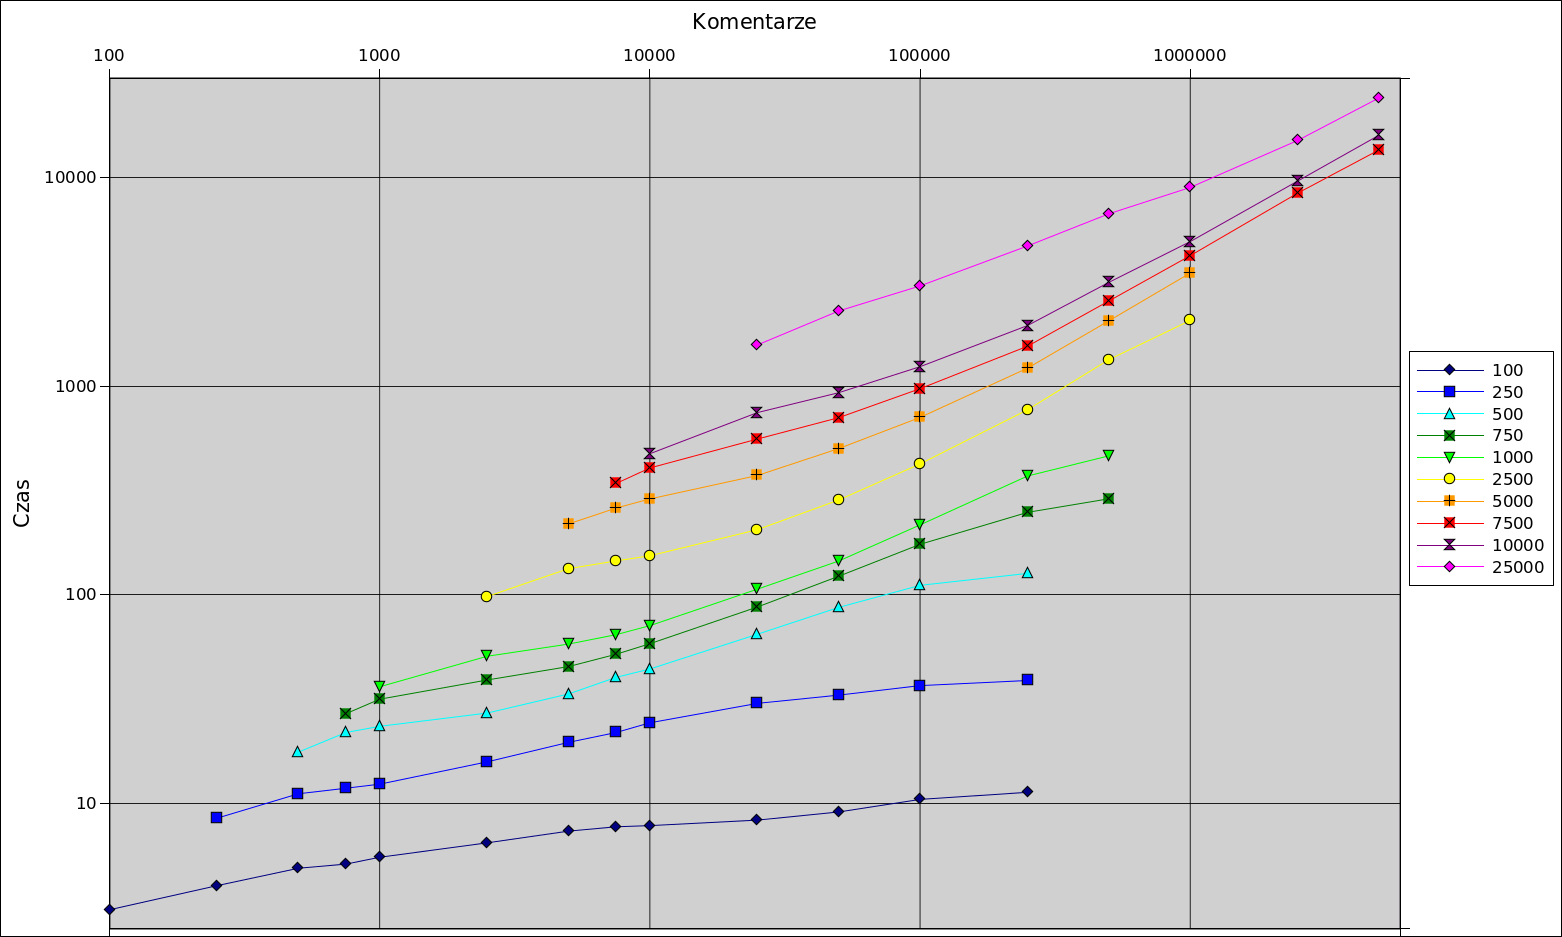
\includegraphics[width=\textwidth]{Wykres1}
\end{centering}
\subsubsection{Czas od ilości użytkowników}
\textsl{Dla ustalonej ilości komentarzy, dla grup o losowej proporcji, średnia dla 100 wykonań}\\
\begin{centering}
	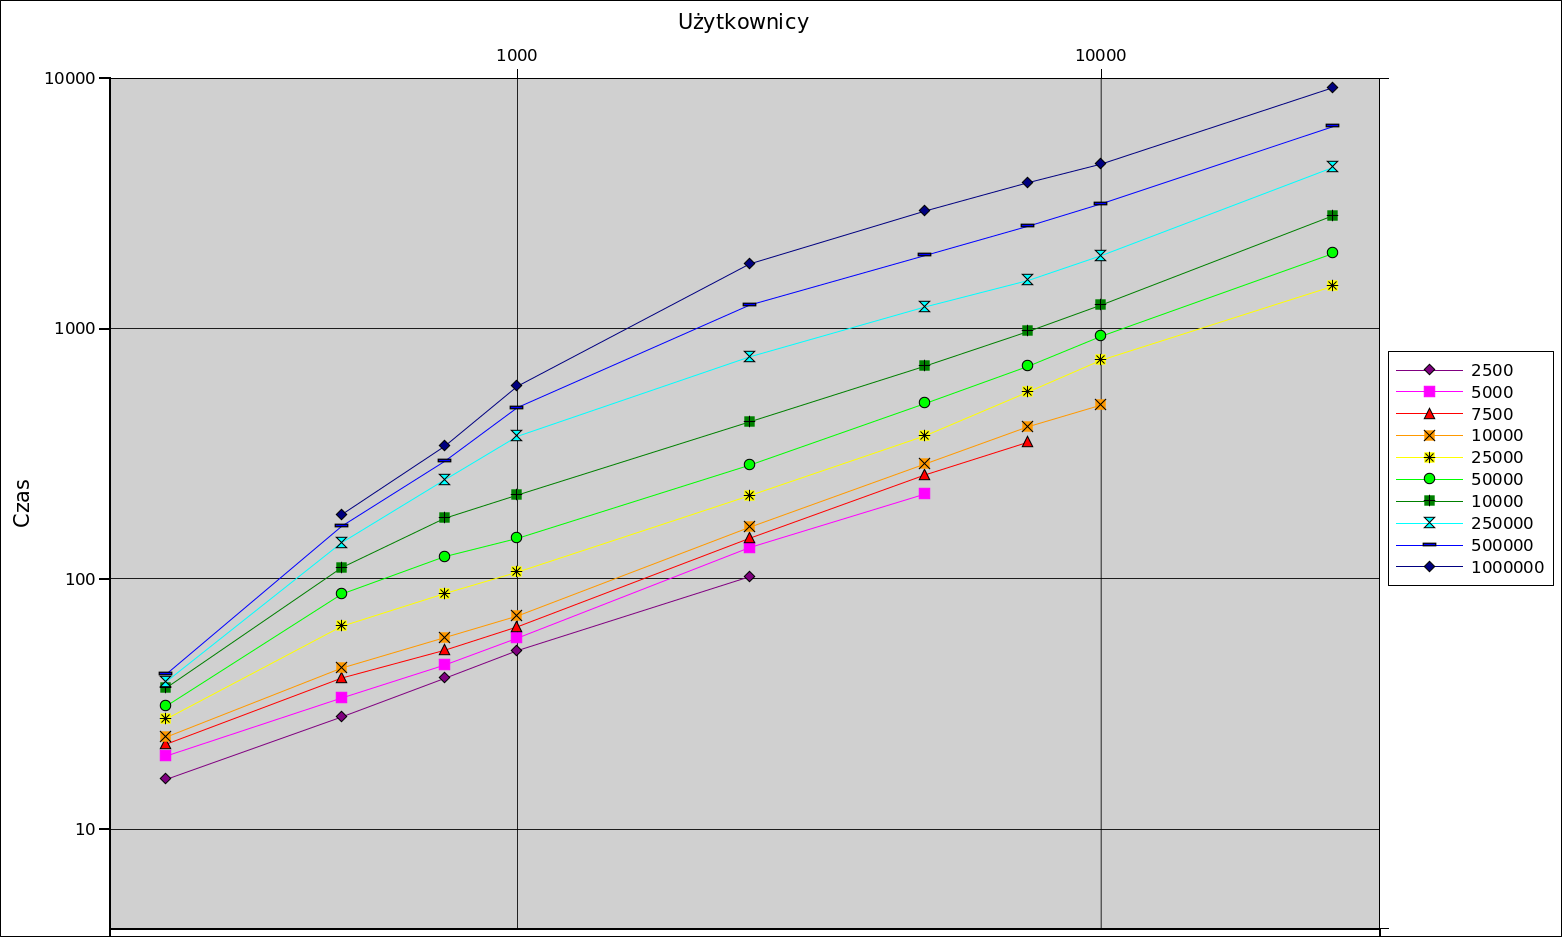
\includegraphics[width=\textwidth]{Wykres2}
\end{centering}
\subsubsection{Czas od ilości użytkowników i ilości komentarzy}
\textsl{Prezentacja "górnej" części danych w celu zapewnienia większej czytelności}\\
\begin{centering}
	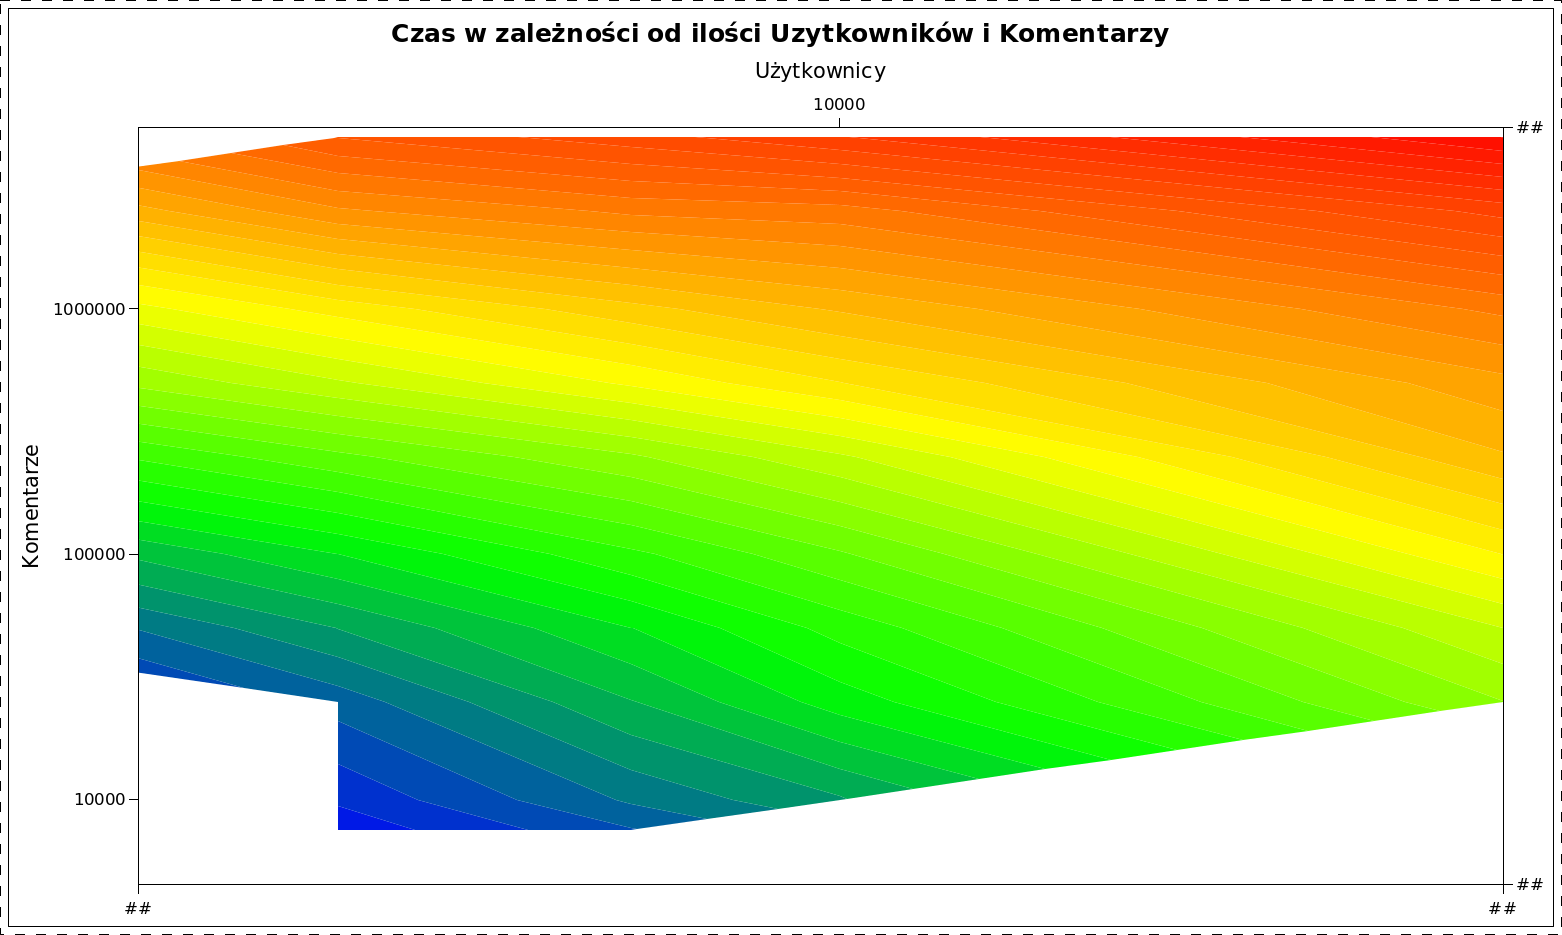
\includegraphics[width=\textwidth]{Wykres3}
\end{centering}
\subsection{Analiza wyników pomiarów}
Przed interpretacją wyników należy zwrócić uwagę na efekt mający wpływ na zmniejszenie czasu obliczeń. Generowania problemów nie uwzględnia tworzenia nieunikalnych połączeń pomiędzy użytkownikami [może wystąpić kilka połączeń pomiędzy 2] które jest niwelowane po wczytaniu problemu do algorytmu skutkując mniejszym rzeczywistym rozmiarem problemu.
\\
Wyniki testów zostały poddane analizie w programie \textit{gnumeric} czego efektem są powyższe wykresy. Ponadto trójki wartości \textit{[liczba użytkowników][liczba komentarzy][czas]} zostały poddane regresji liniowej. Dla regresji wszystkich wartości współczynnik korelacji pomiędzy ilością komentarzy, a czasem \textit{[miarą złożoności problemu]} wynosi : \textit{0.93} co można uznać za złożoność \textit{O(E)} względem liczby krawędzi \textit{E}. Wniosek ten potwierdza obserwacja wykresu.
\\
Dla liczności grupy sytuacja jest nieco bardziej złożona ponieważ korelacja dla całego zbioru wartości wynosi \textit{0.66} co nie dowodzi zależności liniowej. Jednak  
obserwując wykres widzimy, że dla odpowiednio dużych wartości stopniowo wypłaszacza się i ma skośną asymptotę liniową.
\\
Ponieważ zależność pomiędzy złożonością a \textit{E} i \textit{V} jest liniowa to wynikowa złożoność może przedstawiać się jako \textit{O(V*E)} lub \textit{O(V+E)}. Analiza z użyciem regresji liniowej dla 2 zmiennych, próbek o liczbie użytkowników większej od 250 daje zbieżność na poziomie \textit{0.97} 
\\ 
Podsumowując: przeprowadzony eksperyment dowodzi, że zaproponowany algorytm ma pesymistyczna złożoność \textit{O(V+E)} jednak obserwując można zauważyć, że w miarę wypełniania grafu dynamika wzrostu maleje. Ze względu na skończoną liczbę możliwych unikalnych połączeń czas wysyca się w miarę dążenia do grafu pełnego dwudzielnego. wszelkie zduplikowane połączenia śa pomijane w fazie ładowania problemu do programu.
\subsection{Tabela zgodności z przewidywaniami}

\begin{table}[]
	\begin{tabular}{|l|l|l|l|l||l|}
	\hline
	\textit{l.uzytkowników} & \textit{śr. komentarzy } & \textit{l.komentarzy} & \textit{wartość} & \textit{wartość} & \textit{\textbf{pomiar/}} \\
						    & \textit{na użytkownika}  &				   & \textit{przewidziana}	& \textit{pomiaru}   & \textit{\textbf{przewidywanie}}							\\
	\hline
	5000                    & 1.5                               & 7500                      & 702                           & 390.351                  & 0.556                                  \\
	5000                    & 2                                 & 10000                     & 711                           & 398.638                  & 0.561                                  \\
	2500                    & 2                                 & 5000                      & 330.5                         & 190.315                  & 0.576                                  \\
	25000                   & 2                                 & 50000                     & 3755                          & 2606.098                 & 0.694                                  \\
	10000                   & 2.5                               & 25000                     & 1490                          & 938.633                  & 0.63                                   \\
	1000                    & 2.5                               & 2500                      & 104                           & 67.353                   & 0.648                                  \\
	2500                    & 3                                 & 7500                      & 339.5                         & 200.814                  & 0.591                                  \\
	7500                    & 3.33                              & 25000                     & 1127.5                        & 696.972                  & 0.618                                  \\
	750                     & 3.33                              & 2500                      & 67.75                         & 47.304                   & 0.698                                  \\
	2500                    & 4                                 & 10000                     & 348.5                         & 213.9                    & 0.614                                  \\
	25000                   & 4                                 & 100000                    & 3935                          & 3218.993                 & 0.818                                  \\
	5000                    & 5                                 & 25000                     & 765                           & 490.326                  & 0.641                                  \\
	1000                    & 5                                 & 5000                      & 113                           & 75.008                   & 0.664                                  \\
	10000                   & 5                                 & 50000                     & 1580                          & 1095.701                 & 0.693                                  \\
	7500                    & 6.67                              & 50000                     & 1217.5                        & 830.098                  & 0.682                                  \\
	750                     & 6.67                              & 5000                      & 76.75                         & 55.681                   & 0.725                                  \\
	1000                    & 7.5                               & 7500                      & 122                           & 82.002                   & 0.672                                  \\
	2500                    & 10                                & 25000                     & 402.5                         & 267.625                  & 0.665                                  \\
	1000                    & 10                                & 10000                     & 131                           & 89.239                   & 0.681                                  \\
	5000                    & 10                                & 50000                     & 855                           & 592.629                  & 0.693                                  \\
	750                     & 10                                & 7500                      & 85.75                         & 62.96                    & 0.734                                  \\
	10000                   & 10                                & 100000                    & 1760                          & 1356.721                 & 0.771                                  \\
	25000                   & 10                                & 250000                    & 4475                          & 4659.737                 & 1.041                                  \\
	750                     & 13.33                             & 10000                     & 94.75                         & 70.09                    & 0.74                                   \\
	7500                    & 13.33                             & 100000                    & 1397.5                        & 1074.72                  & 0.769                                  \\
	2500                    & 20                                & 50000                     & 492.5                         & 342.313                  & 0.695                                  \\
	5000                    & 20                                & 100000                    & 1035                          & 804.445                  & 0.777                                  \\
	25000                   & 20                                & 500000                    & 5375                          & 6124.138                 & 1.139                                  \\
	1000                    & 25                                & 25000                     & 185                           & 129.983                  & 0.703                                  \\
	10000                   & 25                                & 250000                    & 2300                          & 2031.328                 & 0.883                                  \\
	750                     & 33.33                             & 25000                     & 148.75                        & 107.094                  & 0.72                                   \\
	7500                    & 33.33                             & 250000                    & 1937.5                        & 1646.5                   & 0.85                                   \\
	2500                    & 40                                & 100000                    & 672.5                         & 492.24                   & 0.732                                  \\
	25000                   & 40                                & 1000000                   & 7175                          & 8378.315                 & 1.168                                  \\
	1000                    & 50                                & 50000                     & 275                           & 183.739                  & 0.668                                  \\
	5000                    & 50                                & 250000                    & 1575                          & 1309.985                 & 0.832                                  \\
	10000                   & 50                                & 500000                    & 3200                          & 3161.038                 & 0.988                                  \\
	750                     & 66.67                             & 50000                     & 238.75                        & 159.681                  & 0.669                                  \\
	7500                    & 66.67                             & 500000                    & 2837.5                        & 2628.546                 & 0.926                                  \\
	1000                    & 100                               & 100000                    & 455                           & 286.555                  & 0.63                                   \\
	2500                    & 100                               & 250000                    & 1212.5                        & 891.067                  & 0.735                                  \\
	5000                    & 100                               & 500000                    & 2475                          & 2163.041                 & 0.874                                  \\
	10000                   & 100                               & 1000000                   & 5000                          & 4953.347                 & 0.991                                  \\
	25000                   & 100                               & 2500000                   & 12575                         & 14595.775                & 1.161                                  \\
	750                     & 133.33                            & 100000                    & 418.75                        & 251.623                  & 0.601                                  \\
	7500                    & 133.33                            & 1000000                   & 4637.5                        & 4323.744                 & 0.932                                  \\
	2500                    & 200                               & 500000                    & 2112.5                        & 1476.193                 & 0.699                                  \\
	5000                    & 200                               & 1000000                   & 4275                          & 3684.329                 & 0.862                                  \\
	25000                   & 200                               & 5000000                   & 21575                         & 23649.72                 & 1.096                                  \\
	10000                   & 250                               & 2500000                   & 10400                         & 9808.519                 & 0.943                                 
\\	\hline
\end{tabular}
\end{table}
\end{document}
